
                         \pstart 
           \edtext{\edlabel{dict108v2}Esto altitudo Mercurii \textit{ab} pollices dicti summi \textit{ac} infimi \textit{db} labetur Mercurius ex \textit{ab} vel \textit{aa-bb} ex situ \textit{ac} in situm [\textit{db}]\edtext{}{\Afootnote{\textit{d bb}\textit{\ L \"{a}ndert Hrsg. } }} ita \textit{ac} vel nunc \textit{aa-cc} cadet in \textit{db} et altitudo \textit{b-bb} vel \textit{cc-bb} quam Mercurius labendo percurrit aequalis erit \textit{ab} demta \textit{db}.}{\lemma{dictis.}\xxref{dict108v1}{dict108v2}\Afootnote{ \textit{ (1) }\ Esto altitudo mercurii\protect\index{Sachverzeichnis}{mercurius|textit}   \textbar\ quaecunque \textit{ erg.}\ \textbar\  \textit{ab} vel \textit{bc} vel \textit{aa-bb}   \textbar\ vel \textit{eg} \textit{ erg.}\ \textbar\  
           altitudo pollicum dictorum \textit{ae} vel \textit{fb} vel \textit{bb-g}. Ajo Mercurium\protect\index{Sachverzeichnis}{mercurius|textit} (Tubo existente perpendiculari) semper ex  \textit{(a)}\ situ \textit{ab} perventurum in situm \textit{(b)}\ altitudine \textit{ab} perventurum in altitudinem \textit{aa-bb} ita ut pollices   \textbar\ \textit{ae} vel \textit{ erg.}\ \textbar\  \textit{aa-e} summi succedant in locum infimorum \textit{fb} seu ut  \textit{(aa)}\ linea \textit{(bb)}\ longitudo lapsus \textit{a-aa} vel \textit{b-bb} aequalis sit ipsi \textit{ab} demta \textit{fb}  \textit{(aaa)}\ cumque \textit{bg} \textit{(bbb)}\ seu \textit{bb-g}. Nam si aequalis esset lapsus altitudini \textit{a} pervenisset in \textit{b} et \textit{b} in \textit{g}. Fuisset ergo linea lapsus \textit{bg} cui nunc \textit{bb-g} adimatur. \textit{ (2) }\  Esto [...] \textit{db}. \textit{ L}}}
           \pend 
%Zeitz auskommentiert            %\begin{wrapfigure}{l}{0.1\textwidth}     
% \begin{center}
%  \protect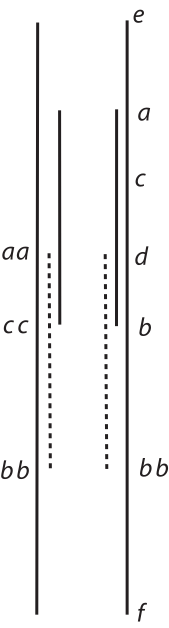
\includegraphics[width=0.2\textwidth]{images/37_3_108v2}%\\\centering{\textit{[Fig. 3]gestrichen}}  
%   \hspace{2cm}            
%                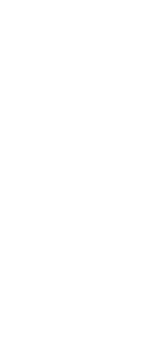
\includegraphics[width=0.2\textwidth]{images/37_3_108v1}\\\textit{[Fig. 3, gestrichen]}\hspace{1.5cm}{\textit{[Fig. 4]}}
%                \end{center}
%                        %\caption{Bildbeschreibung}
%     %                   \end{wrapfigure}
%                        %@ @ @ Dies ist eine Abstandszeile - fuer den Fall, dass mehrere figures hintereinander kommen, ohne dass dazwischen laengerer Text steht. Dies kann zu einer Fahlermeldung fuehren. @ @ @ \\
           \pstart  Hoc necessario eventurum quantacunque sit Tubi in quo Mercurius\protect\index{Sachverzeichnis}{mercurius} descendit longitudo \edtext{aut Mercurii\protect\index{Sachverzeichnis}{mercurius} altitudo}{\lemma{}\Afootnote{aut Mercurii\protect\index{Sachverzeichnis}{mercurius} altitudo \textit{ erg.} \textit{ L}}} facile ostendo. Primum \edtext{longitudo Tubi capacitasque supra}{\lemma{Primum}\Afootnote{ \textit{ (1) }\ non altitudo Tubi capacitasve ultra \textit{ (2) }\ longitudo Tubi capacitasque supra \textit{ L}}} Mercurium\protect\index{Sachverzeichnis}{mercurius} ut \textit{ae} nihil ad rem pertinet, ut praecedentibus experimentis est ostensum. 
             \edtext{Modo Mercurius\protect\index{Sachverzeichnis}{mercurius} non sit 27 (30) pollicibus minor ne atmosphaera\protect\index{Sachverzeichnis}{atmosphaera} ei praeponderet.}{\lemma{}\Afootnote{Modo Mercurius\protect\index{Sachverzeichnis}{mercurius}   \textbar\ non \textit{ erg.}\ \textbar\  sit 27 (30) pollicibus  \textbar\ major, seu \textit{ gestr.}\ \textbar\ minor ne atmosphaera\protect\index{Sachverzeichnis}{atmosphaera} ei praeponderet. \textit{ erg.} \textit{ L}}}
             Deinde nec altitudo Tubi infra Mercurium\protect\index{Sachverzeichnis}{mercurius} quicquam variat, quod facile sic ostendo. Pone Mercurium\protect\index{Sachverzeichnis}{mercurius} pendere in \textit{aa-bb} agglutinetur infimo Tubi orificio \textit{bb} portio nova \textit{bb-f}. Manifestum est, hac additione nihil variari aeris obnitentis pressionem, ergo nec augeri posse descensum. Quantuscunque ergo sit Tubus, fingendum est omnem supra infraque longitudinem ei esse abscissam \edtext{praeter}{\lemma{}\Afootnote{praeter \textit{ erg.} \textit{ L}}} \textit{a-bb} seu spatium quod Mercurius\protect\index{Sachverzeichnis}{mercurius} successive implet. Hinc \edtext{ varia \textso{Experimenta particularia}}{\lemma{Hinc}\Afootnote{ \textit{ (1) }\ varii casus \textit{ (2) }\  varia \textso{Experimenta particularia} \textit{ L}}} consequuntur. Et primum Mercurius\protect\index{Sachverzeichnis}{mercurius} non major altitudine 27 (30) pollicum per nullum plane spatium descendet. \edtext{Imo si minor sit, etiam ascendet posito aerem in Tubo esse dilatatum seu tensum.}{\lemma{}\Afootnote{Imo [...] tensum. \textit{ erg.} \textit{ L}}} Cum enim \edtext{in \textit{db} relinquere cogatur quod hoc spatium impleat, se totum relinquet. Mercurius pollicibus dictis major}{\lemma{enim}\Afootnote{ \textit{ (1) }\ non sit major quam in \textit{db} relinquere cogatur quod hoc spatium impleat, se totum relinquet. Mercurius\protect\index{Sachverzeichnis}{mercurius|textit} \textit{ (2) }\ in [...] major \textit{ L}}} in Tubo supra clauso infra aperto descendens, \edtext{ex tubi summitate}{\lemma{ex}\Afootnote{tubi summitate \textit{ erg.} \textit{ L}}} totus in eo pendulus manebit, nec elabetur, si major sit Tubi longitudo quam est linea \textit{a-bb} seu altitudo Mercurii\protect\index{Sachverzeichnis}{mercurius} duplicata demtis dictis \edtext{\edlabel{poll108v1}pollicibus}{\lemma{}\xxref{poll108v1}{poll108v2}\Afootnote{pollicibus~\textbar\ sumta \textit{ gestr.}\ \textbar\ . Quod \textit{ L}}}.\pend
              \pstart Quod \edlabel{poll108v2}si non labitur ex Tubi summitate, saltem tanta tubi longitudo esse debet ex loco unde labitur si Tubus utrinque clausus est (nam supra apertus infra clausus, aut supra infraque apertus esse non potest). Eadem penitus locum obtinent alioquin enim Tubus Torricellianus\protect\index{Sachverzeichnis}{Tubus!Torricellianus} in aere clauso exhiberi non posset. Hinc patet sine ullo vase stagnante subjecto Mercurium\protect\index{Sachverzeichnis}{mercurius} multis modis pendulum\protect\index{Sachverzeichnis}{pendulum} exhiberi ac proinde Baroscopium\protect\index{Sachverzeichnis}{baroscopium} infra apertum construi posse.\edlabel{poss109r1}
              \pend 
             